\documentclass[11pt]{article}
\usepackage{graphicx}
\usepackage{fancyvrb} 
\usepackage{url}
\title{RSA implementation - Homework \#3 \\ \bigskip \large CNS Course Sapienza}
\date{20th November 2020}
\author{Leonardo Razovic 1712242}
\begin{document}
\maketitle

\section{Introduction}
The \textit{Rivest–Shamir–Adleman} \textbf{(RSA)} cryptosystem revolutionized cryptography when it
emerged in 1977 as the first public-key encryption scheme; whereas classical, symmetric-key
encryption schemes use the same secret key to encrypt and decrypt messages, public-key encryption
(also called asymmetric encryption) uses two keys: one is your public key, which can be used by
anyone who wants to encrypt messages for you, and the other is your private key, which is required
in order to decrypt messages encrypted using the public key.
The RSA algorithm involves four steps: \textit{key generation, key distribution, encryption, and decryption}.
\subsection{Key generation}
The keys for the RSA algorithm are generated in the following way:\cite{rsa-wik}
\begin{itemize}
  \item In order to generate a key, you pick two large prime numbers $p$ and $q$. These numbers have to be picked at random, and in secret.
  \item You multiply them together to produce the modulus $n = p \cdot q$, which is public.
  \item Compute $\lambda(n)$, where $\lambda$ is Carmichael's totient function.\\
        Since $n = p \cdot q$, and $\lambda(n) = lcm(\lambda(p),\lambda(q))$, and since $p$ and $q$ are prime, $\lambda(p) = \phi(p) = p - 1$ and likewise $\lambda(q) = q - 1$.\\
        Hence $\lambda(n) = lcm(p - 1, q - 1)$.
  \item Pick an encryption exponent $e$ (which is also public) such that $1 < e < \lambda(n)$ and $gcd(e, \lambda(n)) = 1$.
        Usually, this value is either $3$ or $65537$. Because those numbers have a small number of $1$'s
        in their binary expansion, you can compute the exponentiation more efficiently.\\
        $(n, e)$ is the public key.
  \item There is a value $d$, the \textit{decryption exponent}, fairly easy to compute assuming that you know $p$ and $q$, such that $d$ is the modular multiplicative inverse of e modulo $\lambda(n)$.
\end{itemize}
\subsection{Key distribution}
Suppose that Bob wants to send information to Alice. Bob must know Alice's public key to encrypt the message and Alice must use her private key to decrypt
the message. To enable Bob to send his encrypted messages, Alice transmits her public key $(n, e)$
to Bob via a reliable, but not necessarily secret, route. Alice's private key $d$ is never distributed.
\subsection{Encryption}
Anyone can use the public key $(n, e)$  to encrypt a message $M$ into a ciphertext $C$ such that $C \equiv M^e (mod \ n)$
\subsection{Decryption}
Using $d$, you can decrypt the message like so: $M \equiv C^d (mod \ n)$
The security of RSA relies on that decryption operation being impossible without knowing the secret
exponent $d$, and that the secret exponent $d$ is very hard (practically impossible)
to compute from the public key $(n, e)$.
\section{Design}
To implement the protocol Rust 1.48.0 has been chosen, with the auxiliary help of several libraries to manage numbers with a high
amount of bit. The main libraries used are:
\begin{itemize}
  \item num-bigint: Big integer types for Rust, BigInt and BigUint.
  \item glass\_pumpkin: A cryptographically-secure, random number generator, useful for generating large prime numbers
  \item openssl: Provdes OpenSSL bindings for the Rust programming language, used to test the encryption/decryption using RSA and AES
\end{itemize}
\subsection{Generate $p$, $q$ and $n$}
The first step is to generate the values of p and q. These two values must be prime numbers, integers, and large enough to be considered safe.
To do this we have chosen to use \Verb"glass_pumpkin" that allows you to generate random prime numbers of a
desired bit length. The randomness comes from the operating system.
Since $p$ and $q$ are values of type \Verb"BigUint" and that this type implements \Verb"Mul" \cite{mul}
it is possible to claculate $n = p \cdot q$.
The length of $n$ in bits represents the length of the key, so if you generate $p$ and $q$ of $512$ bits, you get $n$ at 1024 bits.
The library for generating random prime numbers follows these steps:
\begin{itemize}
  \item Generate a random odd number of a given bit-length.
  \item Divide the candidate by the first 2048 prime numbers. (This helps to eliminate certain cases that pass Miller-Rabin but are not prime.)
  \item Test the candidate with Fermat's Theorem.
  \item Runs $log_2(bit\_length)$ + 5 Miller-Rabin tests with one of them using generator $2$.
  \item Run Lucas primality test.
\end{itemize}
\subsection{Generate $\lambda(n)$}
To compute $\lambda(n) = lcm(p - 1, q - 1)$ where $\lambda$ is Carmichael's totient function, it's possibile to use the \Verb"lcm()" function
provided by \Verb"num_bigint".
\subsection{Generate $e$}
To find $e$ we have two possibilities: use a precomputed value, like $3$ or $ 2^{16} + 1 = 65537$, or
pick a value such that $1 < e < \lambda(n)$ and $gcd(e, \lambda(n)) = 1$. In the code both of the options
are possibile, using the \Verb"gen_biguint_range()" function that generates a random \Verb"BigUint" within the given range, ($1$ and $\lambda(n)$ in our case)
and check if the greatest common divisor between $e$ and $\lambda(n)$ is equal to $1$.
\subsection{Perform Encryption and Decryption}
To perform the encryption of a given plaintext we can use the \Verb"modpow()" provided by \Verb"num-bigint" that returns
(plaintext \^{} exponent $e$) \% modulus $n$ in the encryption
and (ciphertet \^{} exponent $d$) \% modulus $n$ in the decryption phase.
\section{Evaluation}
All tests were performed using Rust 1.48.0 and OpenSSL \cite{openssl} 1.1.1h on Arch Linux running Linux 5.9.8, using an Intel i5 9600KF processor.
To evaluate the correctness and speed of my implementation I compared the results obtained with the results obtained by RSA via OpenSSL.
Each test was performed using Rust's test functions that have been run 20 times, the times reported are an average of the run times.
\begin{table}[h!]
  \centering
  \begin{tabular}{|l|l|l|}
    \hline
    \textit{}                    & \textit{My RSA} & \textit{OpenSSL RSA} \\ \hline
    \textit{Key Generation Time} & \textit{28105}  & \textit{20535}       \\ \hline
    Encryption Time              & 142             & 137                  \\ \hline
    Decryption Time              & 850             & 822                  \\ \hline
  \end{tabular}
  \caption{My implmentantion vs OpenSSL, times expressed in micros}
\end{table}
\\
To speed up the time for encryption and decryption, it is possible to use a smaller exponent $e$, such as $65537$
\begin{table}[h!]
  \centering
  \begin{tabular}{|l|l|l|}
    \hline
    \textit{}                    & \textit{My RSA} & \textit{OpenSSL RSA} \\ \hline
    \textit{Key Generation Time} & \textit{23517}  & \textit{17096}       \\ \hline
    Encryption Time              & 135             & 132                  \\ \hline
    Decryption Time              & 405             & 398                  \\ \hline
  \end{tabular}
  \caption{My implmentantion using a fixed exponent vs OpenSSL, times expressed in micros}
\end{table}
\\
Another test to evaluate the speed was done by comparing the times obtained using AES-128-CBC in OpenSSL,
here we can see very much the slowness of RSA towards AES.
\begin{table}[h!]
  \centering
  \begin{tabular}{|l|l|l|}
    \hline
    \textit{}                & \textit{My RSA} & \textit{OpenSSL AES} \\ \hline
    \textit{Generating Keys} & \textit{25107}  & \textit{0}           \\ \hline
    Encryption Time          & 712             & 650                  \\ \hline
    Decryption Time          & 704             & 638                  \\ \hline
  \end{tabular}
  \caption{My implmentantion vs OpenSSL AES-128-CBC, times expressed in micros}
\end{table}
\\
Using the Linux \Verb"perf" tool it was possible to create a flame graph which shows that most of the time is spent to
generate the keys, especially in checking if the randomly generated numbers are prime.\\
\begin{figure}[h]
  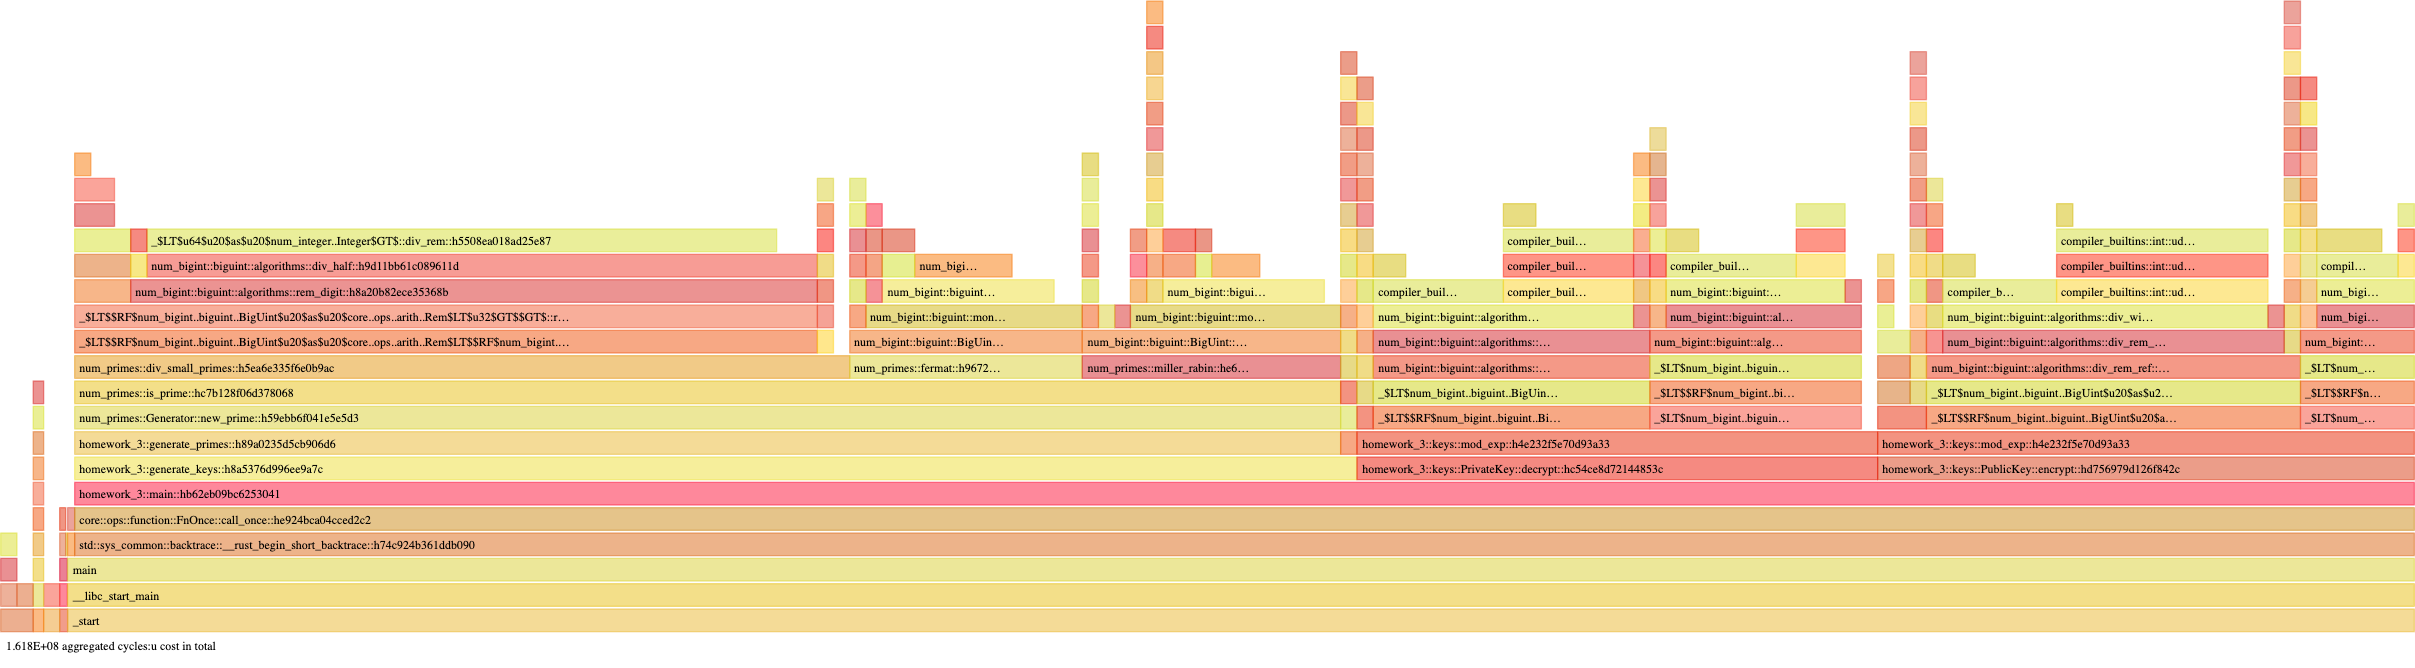
\includegraphics[scale=0.17]{flame.png}
  \caption{The flame graph generated by the complete execution of key generation, encryption, and decryption}
\end{figure}
\section{Conclusion}
In this homework it was possible to study and implement an unsafe, but valid,
version of RSA and compare it with real (and safe) implementations.
The results obtained show how slow an asymmetric scheme, such as RSA, can be, compared to a symmetric scheme, such as AES-128 in CBC mode.

\begin{thebibliography}{9}
  \bibitem{mul}
  Crate num\_bigint documentation.\\
  \url{https://docs.rs/num-bigint/0.3.1/num_bigint/struct.BigUint.html#impl-Mul\%3CBigUint\%3E}
  \\Accessed: 2020-19-11.

  \bibitem{openssl}
  OpenSSL Software Foundation.\\
  \url{https://www.openssl.org/index.html}
  \\ Accessed: 2020-19-11.

  \bibitem{rsa-wik}
  RSA (cryptosystem)\\
  \url{https://en.wikipedia.org/wiki/RSA_(cryptosystem)}
  \\Accessed: 2020-20-11.
\end{thebibliography}
\end{document}
